\section{Evaluation}
In this section of the paper we will evaluate our work in real world applications and determine its strengths and weaknesses. We will use various implementation to perform this evaluation. We will also look into situations where the implementation does not match the protocol description and observe the systems behaviour.

%\subsection{Test Environment}
%For testing our 
\subsection{Chat Server}
To test the capabilities of our DSL, we decided to create a secure chat application. This application would allow  users to connect to the server and exchange secure and private messages with other connected users. We would establish a secure connection to the server and to each individual user that was connected using the DHM key exchange. This means that our Consumer needs to maintain a list of multiple private session keys and be able to determine which one to use for incoming messages.

One of the key benefits of this solution is that even though our central server will receive all the messages, they will be encrypted using two keys. The first key is the one that is established between the two consumers. The second key is the one that the Server and consumer created. This makes it impossible for the server to know what the actual content of the message is. All the server knows is who is talking to who. 

There will be two parts to a message, the headers and the actual text of the chat message. The headers will determine who the intended recipient is. Below we show an example chat message being sent from A to B.
$$
 \begin{multlined}
  \{\{Headers\}, \{Text\}Key_{A2B}\}Key_{A2Server}
 \end{multlined}
$$
Here we can see that the header is only encrypted with key between consumer A and the Server. The text however is encrypted by both the A2Server and A2B key. When the server receives this message, it decrypts it and forwards it to the correct recipient. It however re-encrypts the message using the B2Server key.
$$
 \begin{multlined}
  \{\{Headers\}, \{Text\}Key_{A2B}\}Key_{B2Server}
 \end{multlined}
$$
\\\\
The steps for the connecting client will be 3 steps. 
\begin{enumerate}
 \item Connect to the server and establish a secure communication channel
 \item Register our Username
 \item Receive and send chat messages
\end{enumerate}

Using the steps shown above we can create the protocol description for the server. 
\begin{lstlisting}[style=myScalastyle]
 val endpoint = new ProtocolBuilder()
 val dhm   = endpoint receives primeAndGenerator 
                  sends aPublicKey receives aPublicKey
 val chatServer = dhm receives aUsername 
                       next endpoint anyone aChatMessage looped()
\end{lstlisting}
Here we have re-used our implementation of DHM we defined earlier and added the messages needed for a chat server.

\subsubsection{Detection of Implementation Errors}
The main purpose of our DSL is to discover errors in implementation. When errors occur, we send the error generated by the Validator to the consumer. These errors will provide us with the information  we need to correct the implementation. 

It is up to the consumer to chose how to handle this error. In our implementation we simply print the error message to the terminal. When we run our application, we will be alerted whenever a error occurs and get the information we need to correct it.

We will show two of the errors we received when we where working on the implementation. One of the errors is when our validation failed. 
\begin{lstlisting}[style=myScalastyle]
  ``ValidationError(Msg could not be converted to a PrimeAndGenerator class: ,net.liftweb.json.MappingException: Do not know how to convert JString(239.0) into double)''
\end{lstlisting}
The first part of the message tells us where the error occurred. The second part is the actual exception that was generated. Using the first message we can see that the error ocurred in the message wrapping for PrimeAndGenerator. The exception tells us that we were unable to map ``JString(239)'' to a Double. This level of detail provides us with more than enough details to correct the error.

The second error we had was when our consumer had not implemented a case for the ``PrimeAndGenerator'' class in its the pattern matching.
\begin{lstlisting}[style=myScalastyle]
  ``Unspecified case for: PrimeAndGenerator(149.0,2.0)''
\end{lstlisting}

As we encounter these errors, we can quickly determine their cause and incrementally fix them until we have a running system. In this case we implemented a case for the PrimeAndGenerator where we continued the process defined in our protocol definition.

\subsubsection{Finished System}
After incrementally adding cases to our consumers pattern matching method, we ended up with a fully functioning system. In our implementation we made the clients chose a random integer as a username when connecting. 

The server alerts connected users when a new users connects. When the connected clients receive this ``NewUser'' alert, they establish a secure connection with the new user and send a simple greeting message. Below we have included the screen-shots of three terminals. The terminals represent the server (\ref{fig:server}), client A (\ref{fig:clienta}) and client B (\ref{fig:clientb}). In this scenario, client A is first to connect to the server and will send a greeting to client B.

\begin{figure}[H]
  \centering
  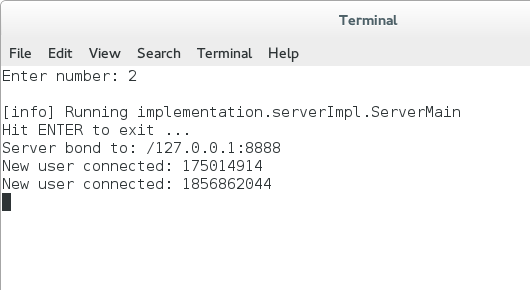
\includegraphics[width=1\linewidth]{evaluation/Server.png}
  \caption{Secure chat server with connected users}
  \label{fig:server}
\end{figure}

\begin{figure}[H]
  \centering
  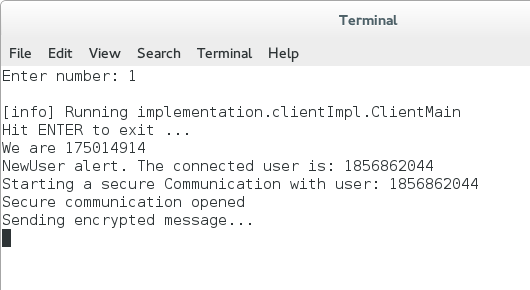
\includegraphics[width=1\linewidth]{evaluation/ClientA.png}
  \caption{Client A - Sends message}
  \label{fig:clienta}
\end{figure}

\begin{figure}[H]
  \centering
  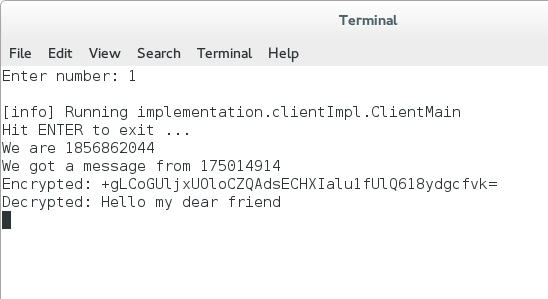
\includegraphics[width=1\linewidth]{evaluation/ClientB.png}
  \caption{Client B - Receives message}
  \label{fig:clientb}
\end{figure}

Any additional clients that connect to the server will also receive greeting messages from both client A and B.

%ServerSide => Unspecified case for: PrimeAndGenerator(149.0,2.0)

%ClientSide => ValidationError(Msg could not be converted to a PrimeAndGenerator class: ,net.liftweb.json.MappingException: Do not know how to convert JString(239.0) into double)


%Server Username => Unspecified case for: LPO2gbvztUktNyx5+BIsidWgBKslDau969BoddEUcs8=
\subsubsection{Network packages}
We will ensure that the values sent over the network truly are what we expect them to be. We do not want to be sending unencrypted values thinking they are encrypted.  For verifying what the values are, we will use the network analyzer Wireshark. Wireshark will capture and save the packets that are sent over the network. We will then be able to read the data that is sent over the network.

In the figures below we show the data that Wireshark has captured. This is the data that has been sent to and from the server. The colours of the text alternates between red and blue. This is to separate the multiple messages and make it clear who the sender of each message. In this case red represents the client while blue is the server.

The first figure is between the Server and Client A (\ref{fig:wsclienta}), while the second is the Server and Client B (\ref{fig:wsclientb}).

\begin{figure}[H]
  \centering
  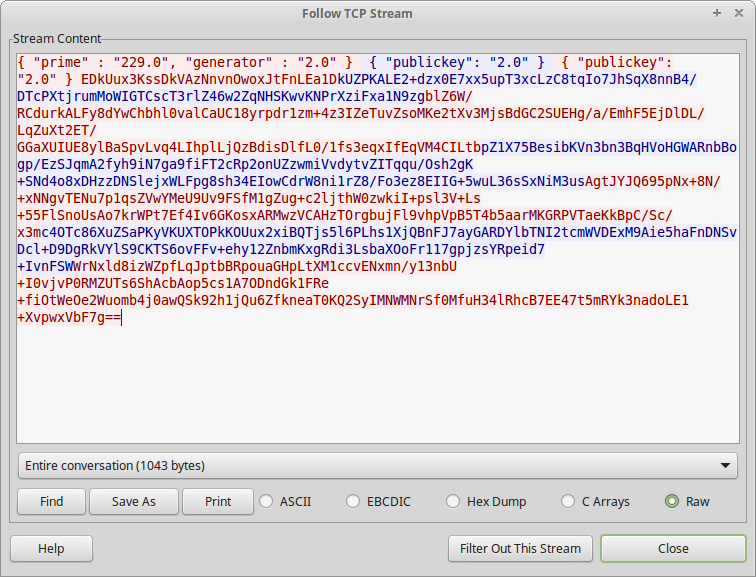
\includegraphics[width=0.9\linewidth]{evaluation/WSClientA.png}
  \caption{Client A packets with server}
  \label{fig:wsclienta}
\end{figure}

\begin{figure}[H]
  \centering
  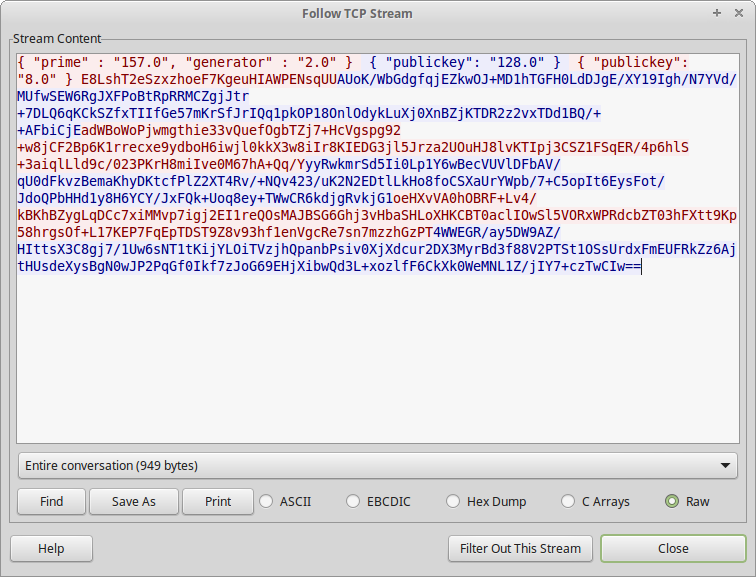
\includegraphics[width=0.9\linewidth]{evaluation/WSClientB.png}
  \caption{Client B packets with server}
  \label{fig:wsclientb}
\end{figure}
We can see that the first messages sent are the ones to establish a DHM key exchange. After the final public key has been sent, all future communication is encrypted. This confirms that the encryption is working as intended.

\subsection{Measuring the performance of echo servers}
To measure the performance of our system, we have decided to implement echo servers that both use and don't use our system. The reason we have not run the performance test on a more complicated system is the same reason why we created this DSL. Implementing a complex solution that uses the bare minimum of features would require a lot of time and effort. Unfortunately those are both scarce resources that are better spent elsewhere. In addition, the numbers that we generate from these experiments should hold true for more complex protocol implementations. 

By using our DSL we will check if every single message sent or received obeys a given protocol. This involves checking that the message contents and protocol specification are of an expected value. These extra steps do not come for free and the overall throughput of the system should be lower than that of a system with no such checking. 

To test this we have created 3 implementations that all build upon the previous implementation. The implementations will be on the server side and will all provide an echo server. The three implementations are the following:

\begin{description}
  \item[Basic] does not use a PM and sends data directly to the consumer
  \item[Uses PM] uses our PM with a simple String Validator
  \item[Wrapping] the Validator wraps messages into an EchoMessage class
\end{description}
We have created a client that measures the time it takes to send and receive a given amount of messages.

The data below shows the average scores for the implementations. As there is some overhead costs when connecting to the server and sending the first message, we do not disconnect and reconnect for each iteration. Instead, we count the time it took to receive the first 10000, 20000, 30000 etc. messages. We gathered results from 20 such iterations. The results below in table \ref{tab:performance} are the averages for each iteration. The time is given in milliseconds. 

\begin{table}[h]
	\centering
	\begin{tabular}{|l|l|l|}
		\hline
		{\bf }         & {\bf Average} & {\bf Message/ms} \\ \hline
		{\bf Basic}    & 489           & 20.40              \\ \hline
		{\bf Uses PM}  & 544           & 18.37              \\ \hline
		{\bf Wrapping} & 589           & 16.37              \\ \hline
	\end{tabular}
	\label{tab:performance}
	\caption{Average performance of implementations given in milliseconds}
\end{table}
% Uses PM is perhaps the most comparable one
If we look at the data we can see quite clearly that there is a performance penalty when using our system. Analyzing the performance table we can see that the throughput of the system is reduced by approximately 4 messages in the full implementation that uses wrapping. Sending 10000 round-trip message that bypasses the PM took an average of 489 milliseconds. Messages that went through the PM and were wrapped took on average 589 milliseconds. This is an increase of approximately 20\%. In many application this increase could potentially be unacceptable.

\subsubsection{Analysing the performance drop}
The reason why the Basic implementation is faster is that it does not need to read the data it receives. It simply returns whatever it receives, without needing to look at the contents. The other implementations need to perform several additional steps than just echoing the message:
\begin{enumerate}
  \item Check if receiving is according to the protocol state
  \item Update protocol state
  \item Convert the message to a String 
  \item Validate the message
  \item Send validated message to the Consumer
  \item Generate and send response
  \item Check if sending is according to the protocol state
  \item Validate the message
  \item Update protocol state
  \item Convert message to a ByteString
  \item Send the message
\end{enumerate}
As we can see there are quite a few additional steps involved in our system. It seems only natural that the we would suffer from some form of performance loss.

We feel however that a 20\% cost is acceptable for most applications as we are comparing it to a system that has no checking and does not abide by any type of protocol. In addition, this DSL is not focused on performance, but increasing readability, maintainability and helping with the implementation.

If performance is the primary concern of a system, you can still reap benefits from the usage of the DSL. In a scenario where you want a server to have high performance as well as protocol compliance, you can verify that it obeys a protocol by using a Protocol Monitor on the opposite end. In this case you can create a client that can interact with the server and the clients Protocol Monitor will generate an error if the protocol is not honored by the server.  


\subsubsection{Concurrency}
One of the objectives when building the DSL was so it would be concurrent. To test this we will use the HTTP server we created in section \ref{sec:httpserver} HTTP Server. To do the actual tests we will use the library Gatling\footnote{\href{www.gatling.io}{gatling.io}}. Gatling gives us a DSL to emulate a user navigating a web page. These steps of navigation is referred to as a ``scenario''. The scenario we have created is a user connecting to the homepage, navigating to the`` test1'' page then finally navigating to the ``test2'' page. In between each navigation we will pause 1 second. The amount of users connecting to server will be slightly more complicated than the scenario. We will start with 100 users connecting to the server, then add 50 000 new users over the next 30 seconds. This is approximately equal to 1667 new users connecting to the server per second. When a user has finished the scenario, it will disconnect. 

The reason we are using these numbers is mainly because of the limitations on our operating system. Using a combination of numbers higher than what we have set, would generate an error specifying that we were not allowed to open any addition file: ``java.net.SocketException Too many open files''. This is a limitation of the OS and not our system. The numbers we have specified should however provide proof of the system being concurrent, although they do not show the max potential and breaking point of the system. It should also be noted that these numbers are dependent on the hardware they are run on. For the results below we have used a standard laptop with a Intel Core 7 processor and 8GB of RAM.

\begin{figure}[H]
  \centering
  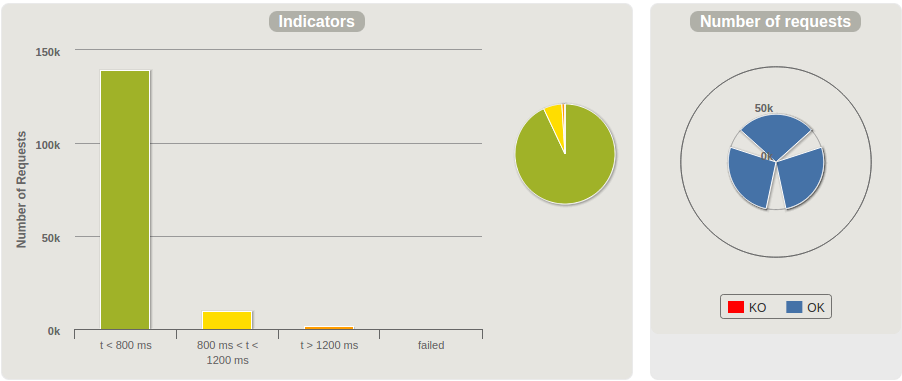
\includegraphics[width=0.9\linewidth]{evaluation/Latency.png}
  \caption{Concurrency - Request latency}
  \label{fig:latency}
\end{figure}
In figure \ref{fig:latency} we can see the latency of the requests. The majority of the requests were below 800ms, with only a few above. We can also see that none of the requests failed, this means that none of the requests were dropped and all were fulfilled.

\begin{figure}[H]
  \centering
  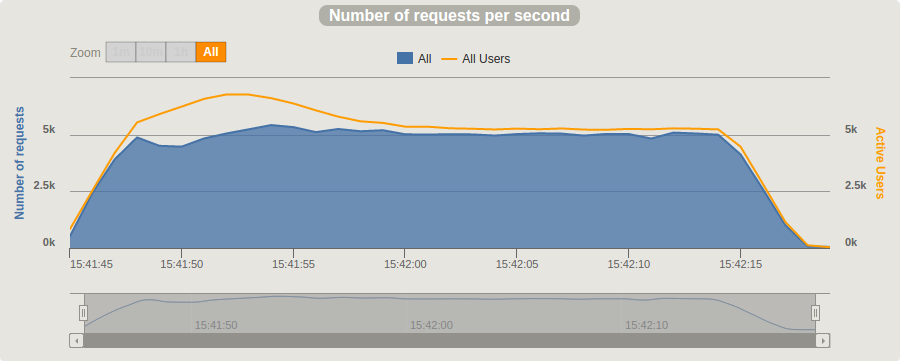
\includegraphics[width=0.9\linewidth]{evaluation/RequestsPerSecond.png}
  \caption{Concurrency - Requests per second}
  \label{fig:requestspersecond}
\end{figure}
In figure \ref{fig:requestspersecond} we can see the number of requests with the number of active users. The request to users is nearly at a 1:1 ratio. We do however see this does not hold true for when the amount of active users is above 5000. This may be due to the limit of requests set by the operating system or it may be the actual max capacity of our system. 

\begin{figure}[H]
  \centering
  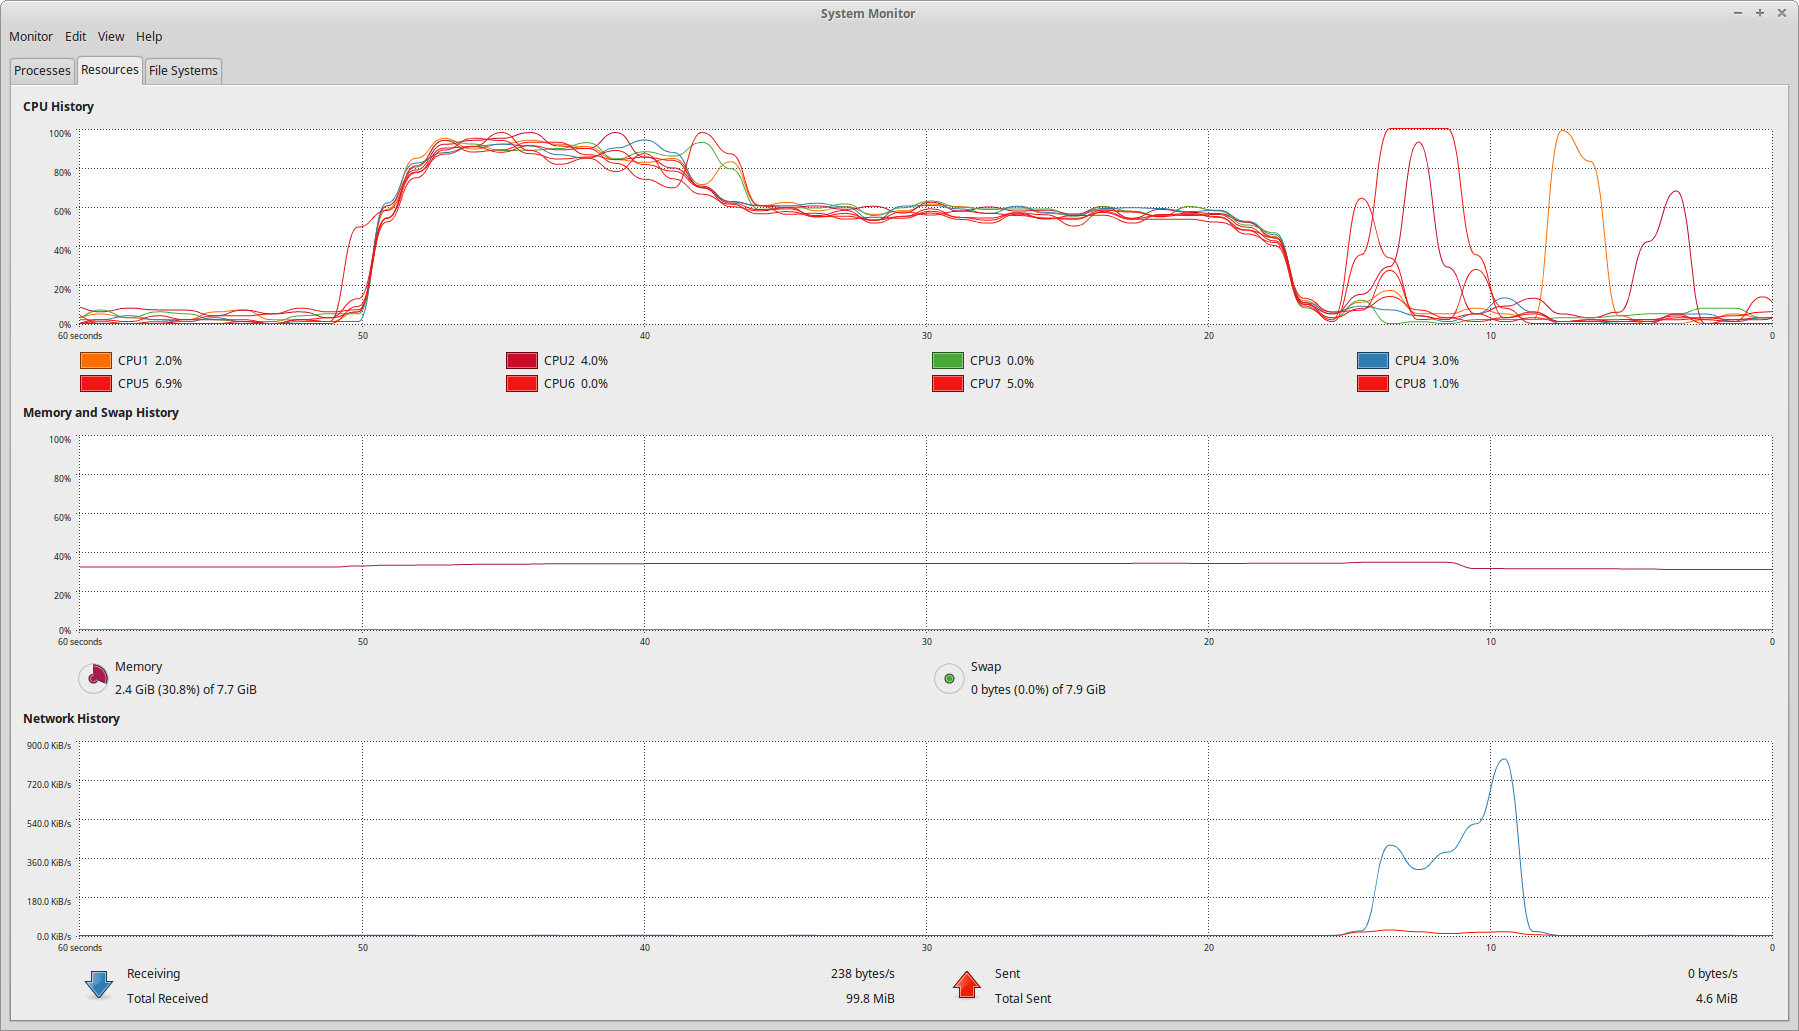
\includegraphics[width=1\linewidth]{evaluation/Monitor.png}
  \caption{Concurrency - System Monitor}
  \label{fig:monitor}
\end{figure}
In figure \ref{fig:monitor} we have the System Monitor that shows the usage of the CPU cores. We can clearly see when the stress test begins  and when it ends. All eight cores are being equally and fully utilized, showing that the workload is being correctly distributed. We see that the CPU load takes a similar shape as the amount of concurrent users in the previous figure. This leads us to believe that figure \ref{fig:requestspersecond} is representative of the systems max output as the CPU load is near 100\%.

The final CPU work we see at the very end is Gatling generating some of the figures displayed above.

\\\\
The numbers we have presented here should provide proof of our system being able to handle a large amount of simultaneous requests without any real issue.
\subsection{Bug Discovery}
\subsubsection{Echo server performance tests}
While running performance test we stumbled upon what we believed to be a bug inside the DSL itself. After the performance testing client had sent around 70 000 messages to the server, it would have a protocol failure. The error was that the server was receiving a message, while the protocols state was in a sending state. We found this strange as the client only sends a message after it has received a message. As our test client was such a simple implementation, we believed the error was perhaps located somewhere within the DSL.
 
After some debugging of the system, we discovered that the bug was in fact withing the testing client. In our implementation we were accidentally sending an extra message to the server when restarting our counter. After several restarts, the accumulated additional messages would eventually arrive before the server had sent a response.

This error was not discovered when we tested the ``Basic'' implementation, so we had to rerun our performance test for it. This error was only discovered as we were stress testing the system and would most likely not have of been caught if were sending a lower amount of messages.

\subsubsection{Apple's Goto bug}
Apple's goto bug , Formally labeled as ``CVE-2014-1266'' \cite{bland2014finding} is a bug that occurred because of the duplication of a single line of code.  in Apples SSL can be quickly summarized as the error of duplication of a single line of code. This duplicated line of code prevented a security check from being run. A simplified version of the code can be seen below.

\begin{lstlisting}[style=myScalastyle]
if ((err = SecurityCheck1())) != 0)
         goto fail;
         goto fail; // duplicated line
if ((err = SecurityCheck2()) != 0) // dead code
         goto fail;
\end{lstlisting}

This duplicated line causes the ``SecurityCheck2()'' to never be run. The indentation makes it appear to belong to the first ``if'' statement, but the if statement has no curly braces. If statements without curly braces will only include the first line in the if statement.  In this particular case, skipping the final security check would allow for a man-in-the-middle attack.

The actual cause of why this duplicated line was created was most likely due to a merge gone wrong\footnote{Difference of source after merge: \href{https://gist.github.com/hongrich/9176925}{gist.github.com/hongrich/9176925}}. After developers have made changes to the same source file, they will eventually need to combine them. This is often done by merging the two files together. It is highly likely that the duplication occurred in this process.
\begin{figure}[H]
  \centering
  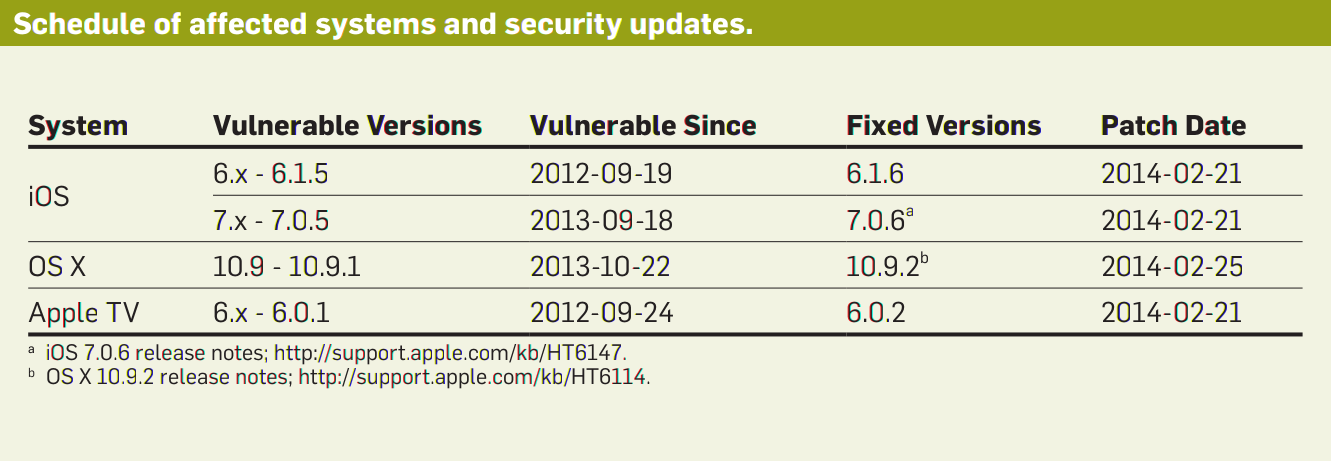
\includegraphics[width=1\linewidth]{evaluation/gotodate.png}
  \caption{Affected systems and patch date of Apple's goto bug \cite{bland2014finding}}
  \label{fig:gotofail}
\end{figure}

There are many questions to how this bug could go unnoticed for so long. In figure \ref{fig:gotofail} we can see that the bug existed for some time before being patched. According to Bland, there are many factors that could of caught this error much sooner:
\begin{itemize}
  \item Coding Standards (indentation, braces)
  \item Code branch merging experience
  \item Code reviews
  \item Coverage data
  \item Compiler warnings
  \item Static analysis warning
  \item Adequate system testing
\end{itemize}

The one that perhaps stands out the most is the fact that the compiler should give a warning when ``dead-code'' is discovered. Dead-code is a term used when a code segment will under no circumstances ever be executed. The SecurityCheck2() should of produced such a warning. Granted you must activate the compiler to show these warnings, but all such errors should always be shown.

The second factor that should of caught this error would be a single unit-test. Landon Fuller has demonstrated that all it would take is 5 lines of code to detect the error\footnote{Landon Fuller's test: \href{https://github.com/landonf/Testability-CVE-2014-1266}{GitHub.com/landonf/Testability-CVE-2014-1266}}.

Bland concludes his article by stating that the error occurred due to a poor development culture within Apple. There are many best practices that they have failed to implement and this resulted in the bug.

Considering the issues described above, I do not believe that the implementation of our DSL would of prevented this bug. It would certainly have of helped as the Validators are easy to use and test. The fact is that the source file that where the bug resides is full of duplicated code. This is something that should of been re-factored during a code review. 

If we assume that the goto bug was included within a Validator, then the Protocol Monitor would not have detected this error. The Protocol Monitor is completely reliant on the implementation of the Validators being correct. If their validate functions contains errors, then the Protocol Monitor will propagate these errors.

%It could of potentially made the error more detectable as the usage of Validators could make testing easier. Apple did however not create a test for their code, even though it would only take 5 lines of code as shown by Fuller. 

Having stated that my system would not have detected Apple's goto bug, I do believe it could of detected similar errors within a different development team. Writing unit tests in general is something that should be done for production ready code. Apple however did not write tests with adequate code coverage and it resulted in this bug. This leads me to agree with Bland's conclusion: The root of this bug lies not within the tools used, but rather in the culture of the development team.

\iffalse
\subsubsection{Heartbleed}
Heartbleed\footnote{\href{http://heartbleed.com/}{Heartbleed's Homepage}} was a weakness discovered within the OpenSSL library that would allow for attackers to read the main memory of a system. OpenSSL is an open source cryptographic library for implementing the Secure Socket Layer (SSL) and Transport Layer Security (TLS). It is used by web servers such as Apache and nginx. Data from a web survey\footnote{http://news.netcraft.com/archives/2014/04/02/april-2014-web-server-survey.html}{Netcraft's Web survey}} conducted by Netcraft in 2014, determined that their combined market share was above 60\% when the bug was discovered.

Heartbleed was such a devastating bug as it was a very simple attack, left no traces of an attack and it was a widespread vulnerability. 
\fi


\subsection{Building DSLs with Scala}
Scala is a powerful language that provides us with much freedom in our creation of a DSL. This freedom is however restrictive in certain areas. Many of these restrictions have been discussed in section \ref{sec:scala} Scala.
 
The perhaps most interesting question when evaluating Scala as a host language for a DSL is to ask if it ever got in the way of implementing our DSL the way we wanted to. To answer this question we consider what we would change in our DSL if Scala did not have any restrictions. At the moment of writing, we do not believe that any of the restrictions that Scala has have affected our implementation negatively. If anything our DSL has not taken advantage of the features offered by Scala. Specifically we could use more implicit values and features such as partial application \cite{odersky2008programming}. 

\subsubsection{DSL or Library}
As we stated in the section above, there are many features of Scala that has not been taken full advantage of when creating the DSL syntax. The primary reason for this is that we have wanted to stay agile to allow for change. Knowedledge that we have gained from implementing protocols has broaden our perspective and insight on implementing protocols. As we have gained this new insight, we have had to change the DSL to increase desirable features and ease of use. Had we created our DSL syntax too early, we would not have been as easily able to facilitate for change.

These are the main reasons why our DSL still feels more like a library, than an actual DSL.
\subsection{Weaknesses}
We have identified what we believe to be some of the main weaknesses with this DSL.

The first is the performance loss of approximately 20\%. The performance test was however slightly unfair as the we compared our system to a system with absolutely no wrapping or any data manipulation. We can therefor consider the 20\% loss as the worst case scenario for similar solutions.

The second weakness is specifying protocols that involve more than 2 participants. By using the Event Bus provided by Akka, we are able to enable communication among the consumers, but this communication channel is not necessarily regulated by a Validator. Sending internal messages that are not defined in the protocol specification can cause undesired side-effects. 

Our final weakness is that there is no indication of error when a consumer should send a message, but is idle. For example, if our echo server does not respond to a echo message, no error would occur. This is because the Protocol Monitor does not know how long it should take to produce a message. The error would have to manually be detected by the the client that would be waitning for the message.

%Even though you implement the DSL, there is no guarantee that it will help debugging the implementation. This is because the strengths of this DSL are heavily dependant on the developers and how they decide to implement a network protocol. Although the use of validators provide a clean way of separating concerns in a system, they must be implemented correctly. Poorly written error messages will not provide useful information when debugging. Validators must try to encapsulate as much of the systems complexity as possible. This complexity should be the focus of determining the purpose of a message and wrapping it in a suitable case class. In most cases, the validator should wrap messages inside classes. This will greatly help building the consumers pattern matching function.


\subsection{Accomplished Objectives}
All the objectives have been met, with the exception of the tertiary ones. One of the secondary objective was to be able to implement additional protocols, specifically the Needham-Schroeder protocol. The main difference of this protocol compared to the Diffie-Hellman-Merkel protocol is that it involves direct communication with multiple clients. With our DHM key exchange, HTTP server and chat server implementations, we only have direct communication with a single client.

To solve multiple connections we must use the Event Bus to communicate with the other actors. In Needham-Schroeder we need direct communication with a server and a client. Figure \ref{fig:Needham} shows an example of how we could implement the protocol. 

\begin{figure}[H]
  \centering
  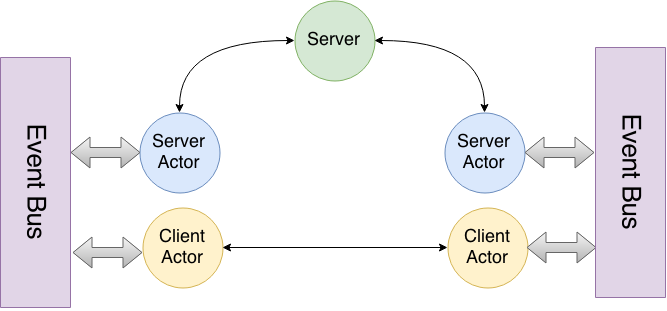
\includegraphics[width=1\linewidth]{evaluation/Needham.png}
  \caption{Needham-Schroeder Actors}
  \label{fig:Needham}
\end{figure}

Here we can create a PM for both the Server and Client actors. This way the PM will be responsible only for communication over a single channel with two participants. The Server and Client actors communicate over the event bus, allowing them to exchange the messages they receive from their connections.

Using similar solutions, we should be able to implement a multitude of different protocols.

 
\iffalse
If you meet your objectives
How did I test it
How do I know its working What happens when it goes wrong
--- Draft 3 ---
How well were the objectives met
What is the performance compared to no checking
-Does not need to quantifiable
How secure it is
How we set out writing it?
"  made this thing using my DSL"
Performance with different message sizes

Speculate on why a sys is slow



Is scala a good language for building a DSL?

This approach definatly has merrits...


Errors: 

ServerSide => Unspecified case for: PrimeAndGenerator(149.0,2.0)

ClientSide => ValidationError(Msg could not be converted to a PrimeAndGenerator class: ,net.liftweb.json.MappingException: Do not know how to convert JString(239.0) into double)


Server Username => Unspecified case for: LPO2gbvztUktNyx5+BIsidWgBKslDau969BoddEUcs8=
\fi

